\chapter{Vizualizácia výsledkov}
\label{chap:FifthChapter}
\begin{hyphenrules}{nohyphenation}
%\todo[inline]{bez nadpisu... potom skuste obrazkom pridat okraj, aby bolo jasne, aka velka stranka je}
Keďže obsahom práce je niečo, čo je veľmi jednoducho vizualizovateľné, a to jednoduchým porovnaním vstupov a výstupov, v ďalšej podkapitole je uvedených niekoľko príkladov. Uvedieme príklady z testovacieho datasetu a aj niekoľko iných dokumentov, ktoré pouvažujeme za zaujímavé na zhodnotenie. Ku každému príkladu uvedieme komentár.
\section{Interpretácia získaných štatistík}
Dosiahnuté výstupné detegované oblasti prezentujeme s dôrazom na~to, ako tieto dáta ovplyvňujú celkové pochopenie problému a efektivitu riešenia. Pre prehľadnosť uvedieme len vybrané strany dokumentov, nakoľko väčšina dokumentov je viacstranová a nie na každej strane sa objavuje anonymizovaná oblasť. Vľavo budeme uvádzať vstup, vpravo výstup.
\newline 

Ako prvé uvedieme príklady, kde detekcia funguje správne podľa očakávaní. Na ďalšej strane na obrázku \ref{fig:5.1} môžeme vidieť, že na dokumentoch, kde bol použitý typ anonymizácie čierny obdĺžník, náš algoritmus presne deteguje tieto miesta.

\begin{figure}[H]
\begin{minipage}[t]{.5\linewidth}
\fbox{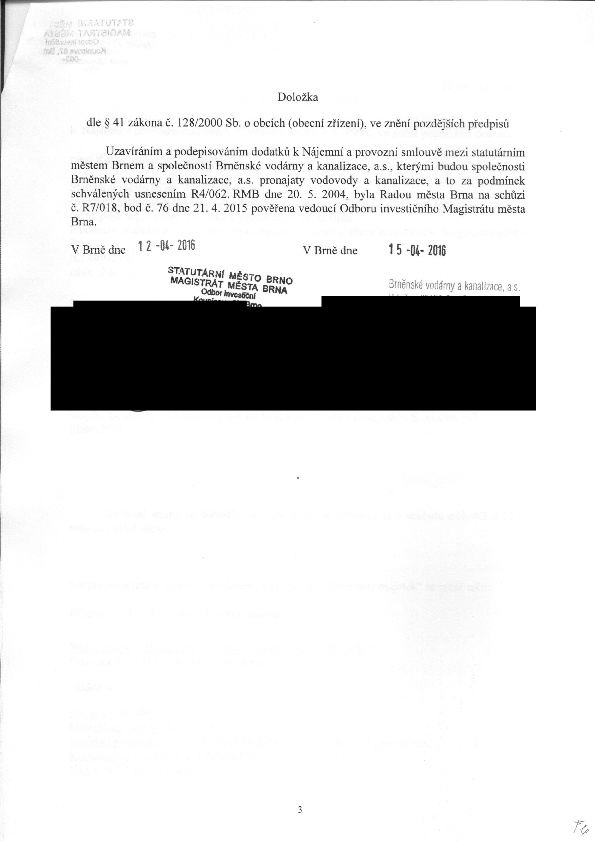
\includegraphics[width=0.9\linewidth]{img/5/03_original.jpg}}
\caption{Percento anonymizovania : 10,61 \%}
\label{fig:5.1} 
\end{minipage}\hfill
\begin{minipage}[b]{.5\linewidth}
\fbox{
\includegraphics[width=0.9\linewidth]{img/5/03_result.jpg}}
\end{minipage}
\end{figure}

Za zmienku tu stojí všimnúť si ľavý horný roh, kde sa vyskytuje relatívne tmavý trojuholník, ktorý vznikol nedokonalým priložením papiera na skener. Náš algoritmus v tomto prípade správne detegoval len miesto, ktoré je naozaj začiernené. Môžeme si všimnúť komplexitu začiernenej plochy. Nejedná sa o~štvoruholník, ale o viac komplexný tvar. V prípade použitia prístupu detekcie bounding boxov by sme museli počítať s tým, že by bol bounding box väčší a~zahŕňal by aj miesta, ktoré začiernené nie sú. To by znamenalo viac algoritmickej práce na overenie, že bounding box naozaj obsahuje len tú plochu, ktorú má a~v~takomto prípade by bolo potrebné rozparcelovať bounding boxy tak, aby dokonale obkreslili nepravidelné tvary. Problém s použitím prístupu bounding boxov by bol ešte viac viditeľný, ak by bola na vstupnom obraze šikmá anonymizovaná oblasť, ako môžeme vidieť v ďalšom príklade na obr. \ref{fig:5.2}.

\begin{figure}[H]
\begin{minipage}[t]{.5\linewidth}
\fbox{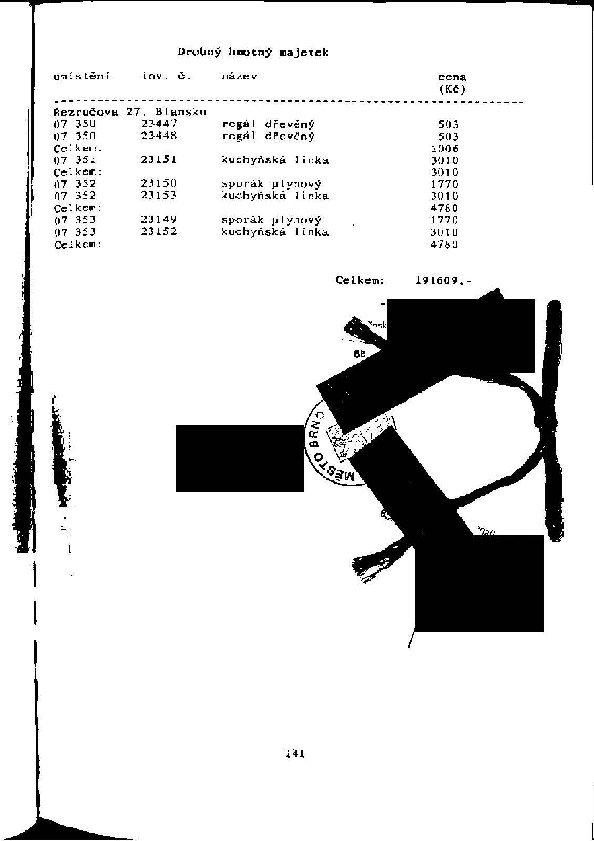
\includegraphics[width=0.9\linewidth]{img/5/73_original.jpg}}
\caption{Percento anonymizovania : 12,68 \%}
\label{fig:5.2} 
\end{minipage}\hfill
\begin{minipage}[b]{.5\linewidth}
\fbox{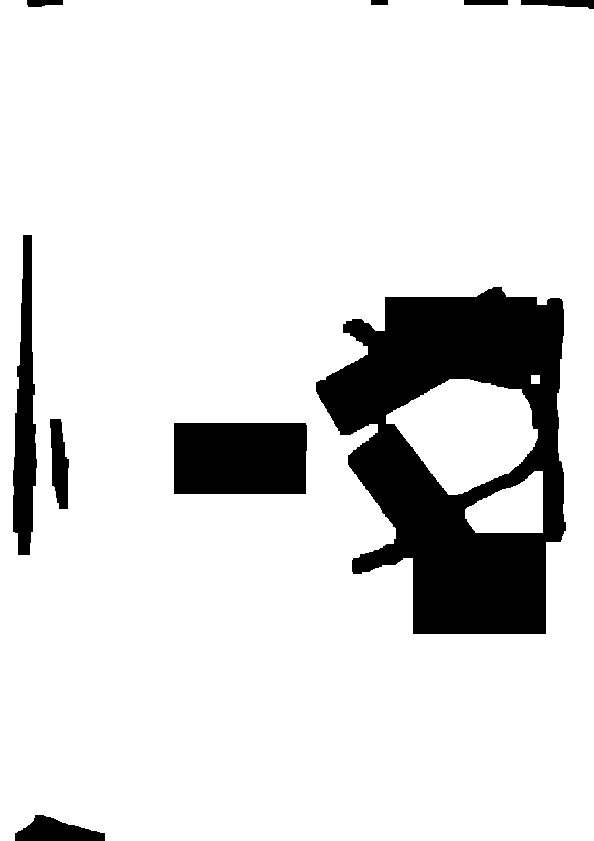
\includegraphics[width=0.9\linewidth]{img/5/73_result.jpg}}
\end{minipage}
\end{figure}

V tomto prípade sa jedná o dokument z roku 1994 a môžeme si všimnúť, že to je nekvalitný sken. V tomto prípade je zobrazená posledná strana a vzhľadom na použitý algoritmus je vidieť, že za anonymizovanú oblasť boli detegované aj oblasti, ktoré nimi reálne nie sú. V tomto konkrétnom príklade bolo pre použitý algoritmus obtiažne rozlíšiť medzi nedokonalosťami skenu, zväzujúcou šnúrkou a najskôr nálepkami prekrývajúce dôležité informácie tohto dokumentu. 
\newline

Jedným z možných riešení by bola detekcia zvislých pozdĺžnych oblastí a~tie vyhodnocovať za chybu. Pri implementácii sme premýšľali nad možnosťami filtrácie, no v tej dobe sme nemohli prísť s rozumným riešením, ktoré by nemalo fatálny dopad na iné analyzované dokumenty, ako si ukážeme na ďalšej strane, na obr. \ref{fig:5.3}.

\begin{figure}[H]
\begin{minipage}[t]{.5\linewidth}
\fbox{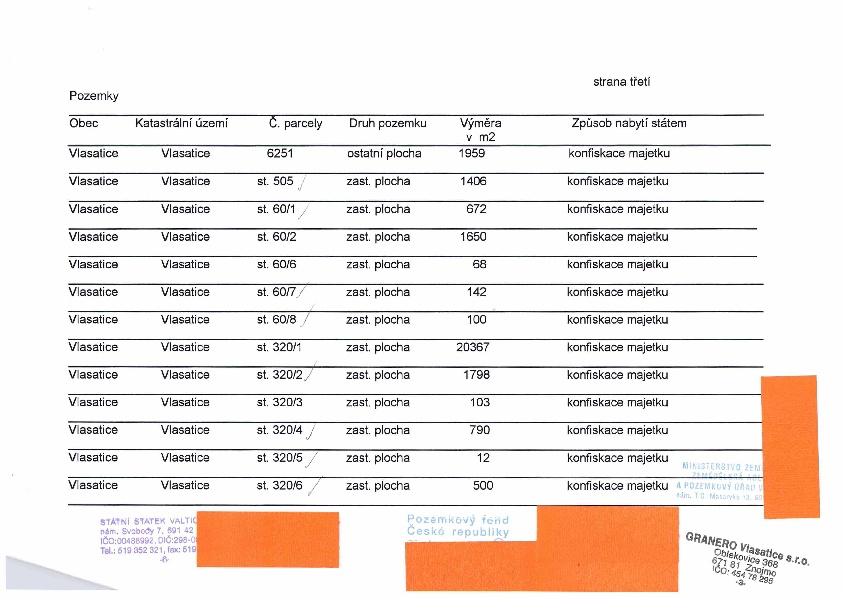
\includegraphics[width=0.9\linewidth]{img/5/9_original.jpg}}
\caption{Percento anonymizovania : 7,45 \%}
\label{fig:5.3} 
\end{minipage}\hfill
\begin{minipage}[b]{.5\linewidth}
\fbox{
\includegraphics[width=0.9\linewidth]{img/5/9_result.jpg}}
\end{minipage}
\end{figure}

V tomto prípade sa jedná o prelepenie farebnými nálepkami, ktoré algoritmus rovnako dokázal detegovať a správne určiť za anonymizovanú oblasť. 
\newline

Na predchádzajúcom príklade sme spomenuli možnú filtráciu pozdĺžnych nepravidelných objektov, čo by v tomto prípade znamenalo detekciu oblasti vpravo od tabuľky (všimnime si, že oblasť nie je zarovnaná a je šikmo) a po následnej filtárcii by došlo k odstráneniu oblasti, ktorá bola pôvodne detegovaná správne. 
\newline

Znovu si môžeme všimnúť celkom výrazného trojuholníka v ľavom dolnom rohu, ktorý náš algoritmus dokázal odfiltrovať a nevyhodnotiť ako tmavú plochu, čo by spôsobilo nesprávne označenie oblasti za anonymizovanú.

\begin{figure}[H]
\begin{minipage}[t]{.4\linewidth}
\fbox{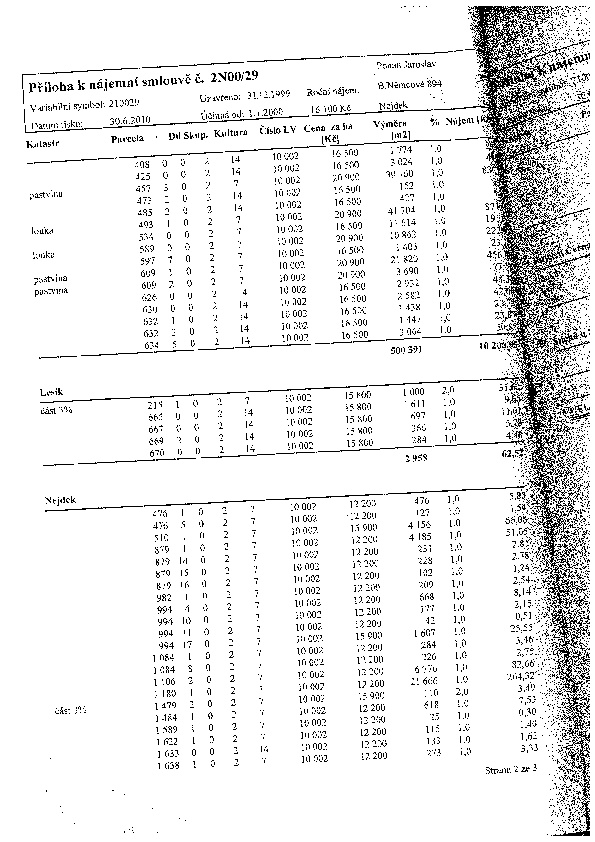
\includegraphics[width=0.9\linewidth]{img/5/4_original.jpg}}
\caption{Percento anonymizovania : 0,08 \%}
\label{fig:5.4} 
\end{minipage}\hfill
\begin{minipage}[b]{.4\linewidth}
\fbox{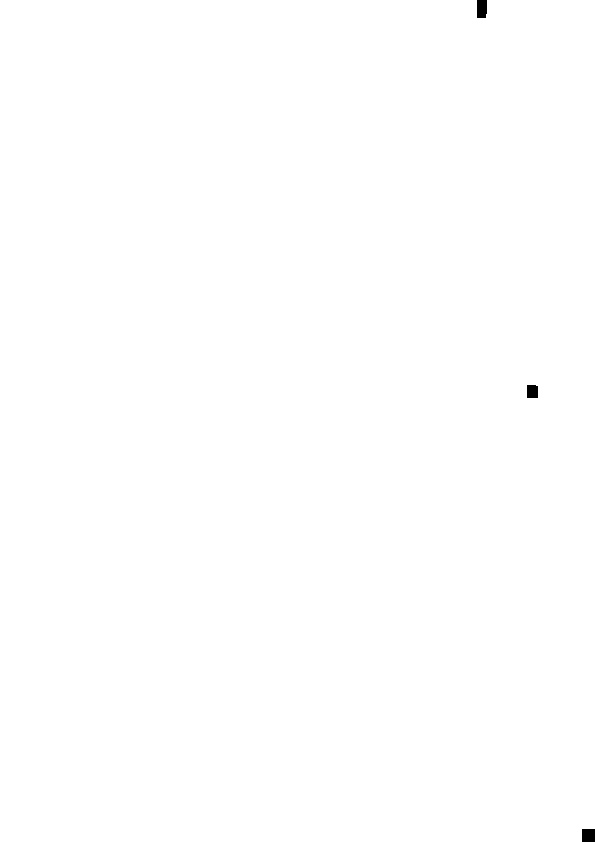
\includegraphics[width=0.9\linewidth]{img/5/4_result.jpg}}
\end{minipage}
\end{figure}

Na obrázku \ref{fig:5.4} vidíme ďalšiu stranu z dokumentu, ktorý bol skenovaný veľmi nekvalitne. V origináli sa síce nevyskytuje anonymizovaná oblasť, no kvôli veľmi zlému skenu boli niektoré oblasti dostatočne tmavé na to, aby boli vyhodnotené naším algoritmom za anonymizované oblasti. Nejedná sa o veľké plochy a možné riešenie takýchto anomálií popisujeme v záverečnej kapitole \ref{chap:conclusion}.
\newline

Na posledných príkladoch si ukážeme tzv. false positives, ktoré algoritmus nebol schopný rozoznať a správne odfiltrovať.

\begin{figure}[H]
\begin{minipage}[t]{.5\linewidth}
\fbox{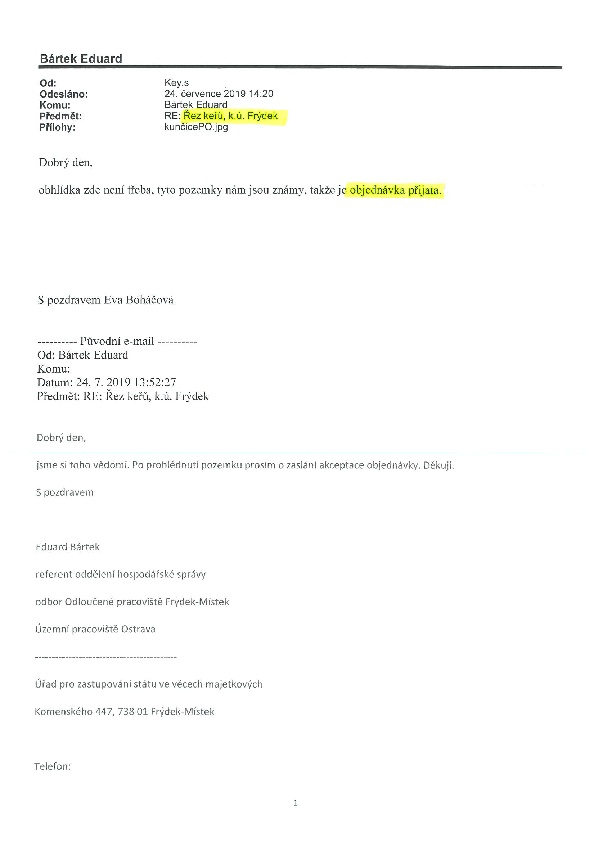
\includegraphics[width=0.9\linewidth]{img/5/3_original.jpg}}
\caption{Percento anonymizovania : 0,07 \%}
\label{fig:5.5} 
\end{minipage}\hfill
\begin{minipage}[b]{.5\linewidth}
\fbox{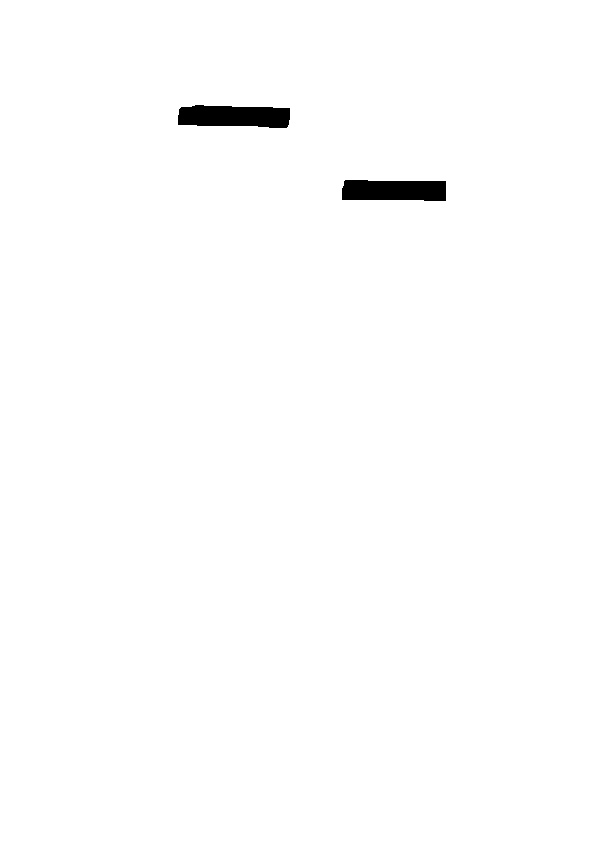
\includegraphics[width=0.9\linewidth]{img/5/3_result.jpg}}
\end{minipage}
\end{figure}

Ako bolo spomenuté v popise algoritmu v \ref{chap:4.1.2}, v prípade detekcie farebných pixelov berieme tieto pixely ako možné anonymizované oblasti. V tomto prípade sa však jedná o zvýrazňovač, no algoritmus to vyhodnotil ako anonymizovanú plochu, a teda tieto oblasti sú false positive. Možné riešenia a prístupy sú spomenuté v záverečnej kapitole \ref{chap:conclusion}.
\newline

Na obrázku \ref{fig:5.6} vidíme obdobný problém, tentokrát týkajúci sa úradnej pečiatky, ktorá je výrazná červená. 

\begin{figure}[H]
\begin{minipage}[t]{.4\linewidth}
\fbox{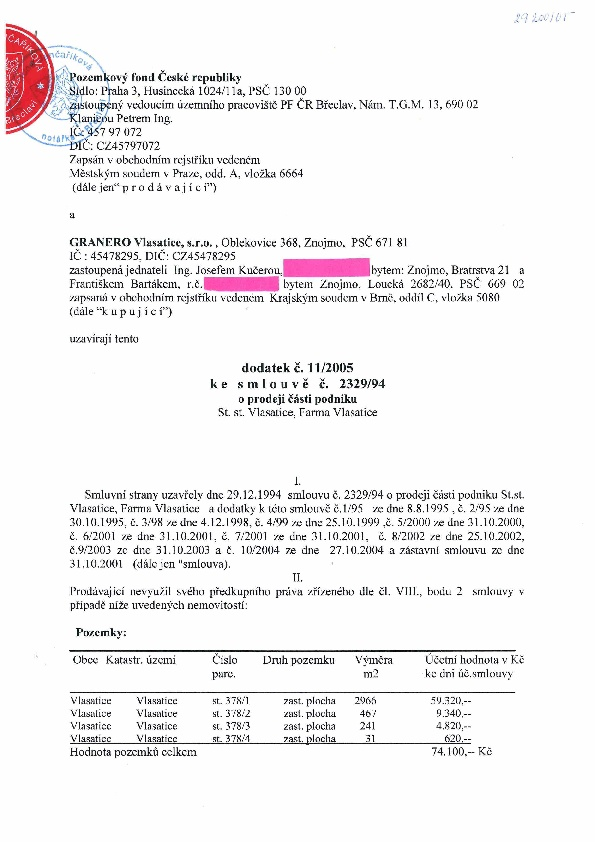
\includegraphics[width=0.9\linewidth]{img/5/1_original.jpg}}
\caption{Percento anonymizovania : 1,4 \%}
\label{fig:5.6} 
\end{minipage}\hfill
\begin{minipage}[b]{.4\linewidth}
\fbox{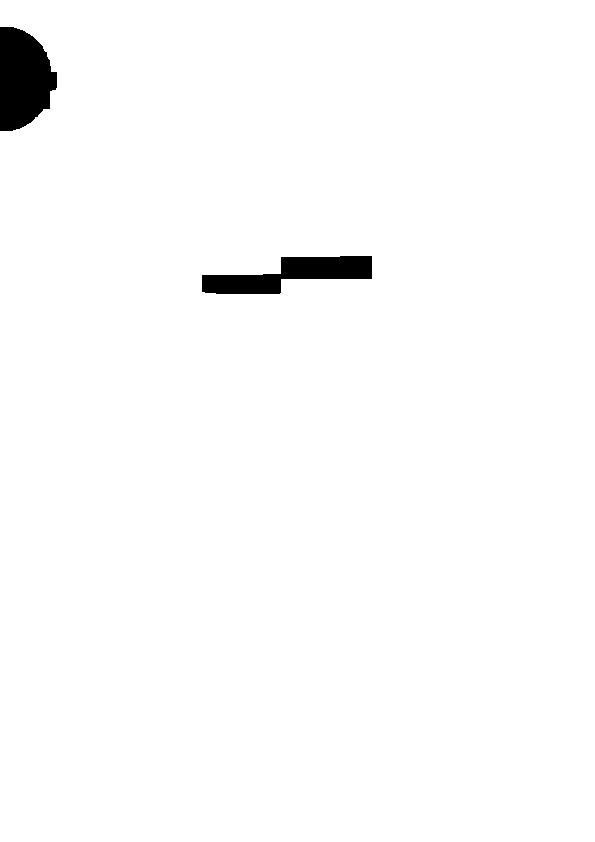
\includegraphics[width=0.9\linewidth]{img/5/1_result.jpg}}
\end{minipage}
\end{figure}

Posledný príklad, ktorý uvedieme (obr. \ref{fig:5.7}), je detekcia anonymizovaných oblastí šumom. Tento typ anonymizácie bol jednym z hlavných problémov, nakoľko bolo veľmi ťažké správne vyfiltrovať bežný šum, ktorý vznikal pri zlom skene od šumu, ktorý prekrýval nejaké údaje a teda sa jednalo o anonymizovanú oblasť. Detegované oblasti nie sú dokonalé, každopádne môžeme prehlásiť, že aj takýto typ anonymizácie sme schopní detegovať a relatívne presne označiť.


\begin{figure}[H]
\begin{minipage}[t]{.4\linewidth}
\fbox{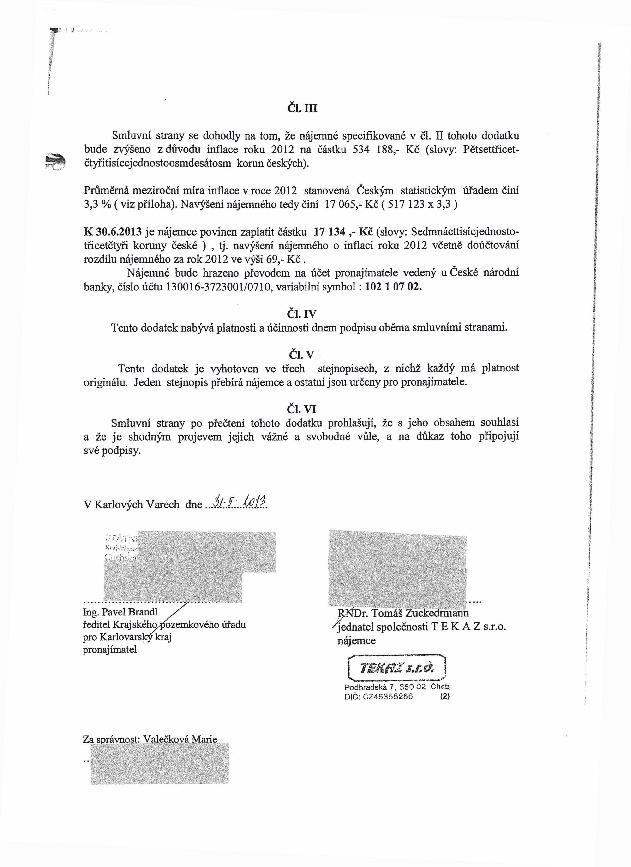
\includegraphics[width=0.9\linewidth]{img/5/2_original.jpg}}
\caption{Percento anonymizovania : 4,2 \%}
\label{fig:5.7} 
\end{minipage}\hfill
\begin{minipage}[b]{.4\linewidth}
\fbox{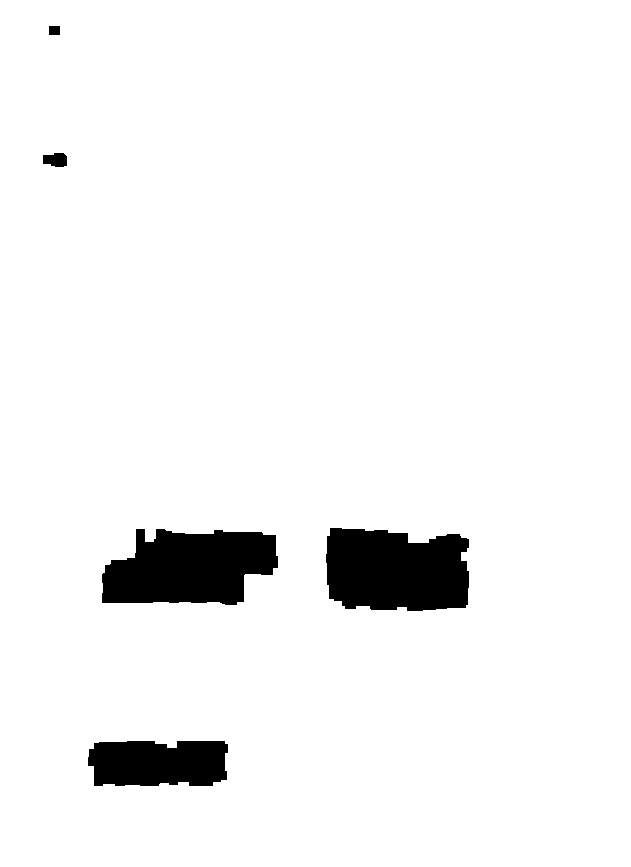
\includegraphics[width=0.9\linewidth]{img/5/2_result.jpg}}
\end{minipage}
\end{figure}

\subsection{Dopady na ďalší vývoj}
Na základe vykonaných pozorovaní a analýz detegovaných oblastí je zrejmé, že algoritmus má schopnosť identifikovať anonymizované oblasti s vysokou presnosťou, zároveň však sledujeme výzvy v špecifických scenároch, ktoré vyžadujú ďalšie vylepšenia. Niekoľko kľúčových poznatkov a návrhov pre ďalší význam, ktoré uvádzame, sú:
\begin{enumerate}
    \item Zlepšenie filtrovacích metód. 
    
    Ako sme si mohli všimnúť v príkladoch s nekvalitnými skenmi, algoritmus má tendenciu označovať tmavé zašumené oblasti za anonymizované. Pre budúci vývoj tak predpokladáme implementáciu pokročilých filtrovacích techník, ktoré by boli schopné dokázať lepšie rozlišovať medzi skutočne anonymizovanými oblasťami a nedokonalosťami skenu.
    \item Rozpoznávanie kontextu. 
    
    Ďalší vývoj algoritmu by mal cieliť na identifikáciu vzorov, kde dochádza k~anonymizácii častejšie a naopak miesta, kde sa anonymizácia spravidla nevyskytuje (napr. okraje strán, nadpisy, určité formáty textov...).

    \item Optimalizácia detekcie tvarov.

    Algoritmus často nesprávne označí zvýrazňovače či farebné pečiatky ako anonymizované oblasti. Budúci vývoj by mal zahrnúť detekciu takýchto tvarov a správne ich identifikovať a ignorovať.
\end{enumerate}
\end{hyphenrules}